
\documentclass[12pt,letterpaper]{article}
\usepackage[utf8]{inputenc}
\usepackage[spanish]{babel}
\usepackage{graphicx}
\usepackage[left=2cm,right=2cm,top=2cm,bottom=2cm]{geometry}
\usepackage{graphicx} % figuras
% \usepackage{subfigure} % subfiguras
\usepackage{float} % para usar [H]
\usepackage{amsmath}
%\usepackage{txfonts}
\usepackage{stackrel} 
\usepackage{multirow}
\usepackage{enumerate} % enumerados
\renewcommand{\labelitemi}{$-$}
\renewcommand{\labelitemii}{$\cdot$}
% \author{}
% \title{Caratula}
\begin{document}

% Fancy Header and Footer
% \usepackage{fancyhdr}
% \pagestyle{fancy}
% \cfoot{}
% \rfoot{\thepage}
%

% \usepackage[hidelinks]{hyperref} % CREA HYPERVINCULOS EN INDICE

% \author{}
\title{Caratula}

\begin{titlepage}
\begin{center}
\large{UNIVERSIDAD PRIVADA-DE-TACNA}\\
\vspace*{-0.025in}
\begin{figure}[htb]
\begin{center}

\includegraphics[width=8cm]{./Imagenes/logo}
\end{center}
\end{figure}
\vspace*{0.15in}
INGENIERIA DE SISTEMAS  \\

\vspace*{0.5in}
\begin{large}
TITULO:\\
\end{large}

\vspace*{0.1in}
\begin{Large}
\textbf{INFORME DE LABORATORIO7} \\
\textbf{Azure Data Studio} \\
\end{Large}

\vspace*{0.3in}
\begin{Large}
\textbf{CURSO:} \\
\end{Large}

\vspace*{0.1in}
\begin{large}
BASE DE DATOS II\\
\end{large}

\vspace*{0.3in}
\begin{Large}
\textbf{DOCENTE(ING):} \\
\end{Large}

\vspace*{0.1in}
\begin{large}
 Patrick Cuadros Quiroga\\
\end{large}

\vspace*{0.2in}
\vspace*{0.1in}
\begin{large}
Integrantes: \\
\begin{flushleft}
Escalante Alanoca Jesus Humberto	\hfill	(2015050641) \\
\end{flushleft}
\end{large}
\end{center}

\end{titlepage}


\tableofcontents % INDICE
\thispagestyle{empty} % INDICE SIN NUMERO
\newpage
\setcounter{page}{1} % REINICIAR CONTADOR DE PAGINAS DESPUES DEL INDICE

\section{Informacion General} 

\begin{itemize}
\subsection{Objetivos:}
	\item Conocer los fundamentos sobre Monitorización de Base de Datos mediante Auditoría.
	\item Poder instalar correctamente  las consultas.
\subsection{ Recursos utilizados:}
	\item Azure Data Studio.
	\item Windows 10 64bit: Pro, Enterprise o Education, con al menos 4GB de RAM.
	\item Microsoft SQL Server 2014 Enterprise

\end{itemize}



\subsection{Azure Data Studio }
Azure Data Studio es una herramienta de base de datos multiplataforma para profesionales de datos que utilizan la familia de plataformas de datos en la nube y locales de Microsoft en Windows, MacOS y Linux.

\begin{center}
		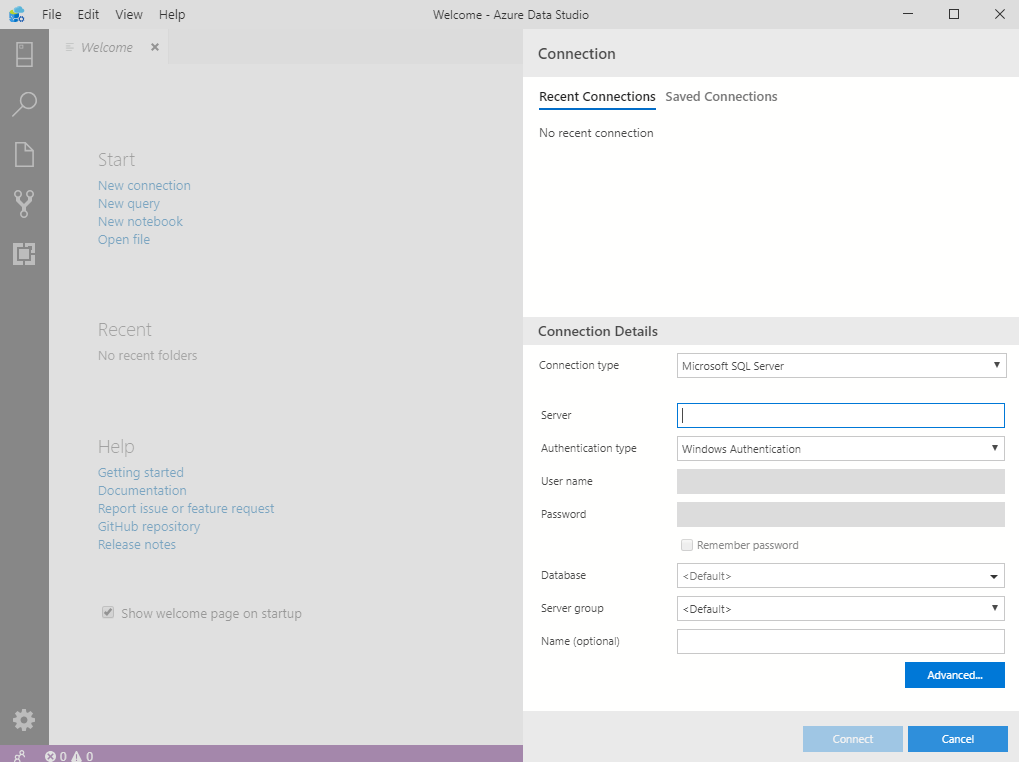
\includegraphics[width=15cm]{./Imagenes/0}
		\end{center}

\begin{center}
		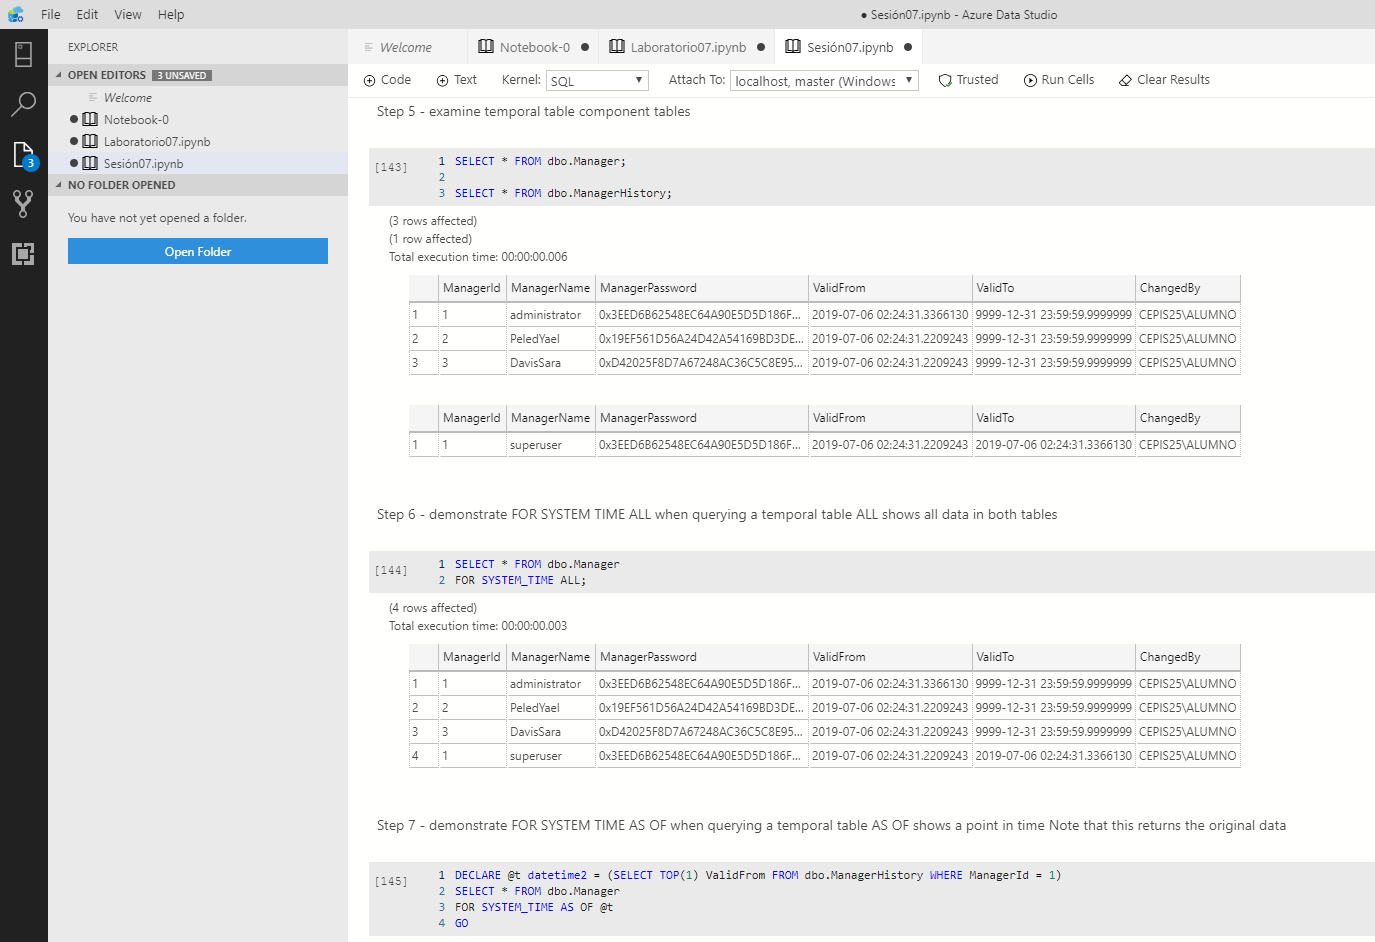
\includegraphics[width=15cm]{./Imagenes/1}
		\end{center}

\begin {itemize}
	\item Editor de código SQL con IntelliSense\\\\
	\subitem Azure Data Studio ofrece una experiencia moderna de codificación SQL centrada en el teclado que facilita sus tareas diarias con funciones integradas, como ventanas de pestañas múltiples, un editor de SQL enriquecido, IntelliSense, finalización de palabras clave, fragmentos de código, navegación de código y control de fuente integración Ejecute consultas SQL .
	\item Fragmentos de código de SQL inteligenter\\
	\subitem -Los fragmentos de código SQL generan la sintaxis SQL adecuada para crear bases de datos, tablas, vistas, procedimientos almacenados, usuarios, inicios de sesión, roles, etc., y para actualizar los objetos de base de datos existentes. Use fragmentos de código inteligente para crear rápidamente copias de su base de datos para fines de desarrollo o prueba, y para generar y ejecutar scripts CREAR e INSERTAR.\\\\
	
	\item Extensibilidad y auditoría de extensión.\\
	\subitem - Mejore la experiencia de Azure Data Studio al ampliar la funcionalidad de la instalación básica. Azure Data Studio proporciona puntos de extensibilidad para las actividades de administración de datos, así como soporte para la creación de extensiones.\\
	
\end{itemize}






\section{Procedimientos} 

\begin{itemize}
\subsection{ Iniciando Docker:}
	\item Abrir el menu inicio y buscar la aplicación Docker for Windows.
                    \begin{figure}[H]
		\begin{center}
		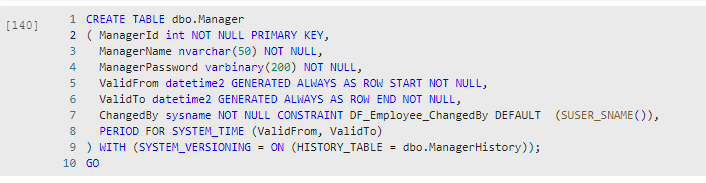
\includegraphics[width=7cm]{./Imagenes/s1}
		\end{center}
		\end{figure}
	\item Una vez iniciado se podrá visualizar el icono de Docker en el área de notificación.
   \begin{figure}[H]
		\begin{center}
		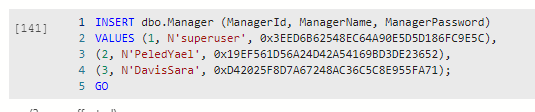
\includegraphics[width=7cm]{./Imagenes/s2}
		\end{center}
		\end{figure}
          \item Asimismo se podrá visualizar la ventana de bienvenida.
          \item Ingresar sus credenciales creadas en Docker Hub para iniciar sesión en el aplicativo..
   \begin{figure}[H]
		\begin{center}
		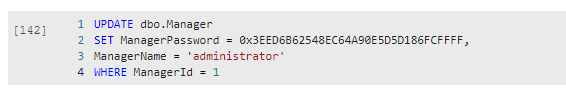
\includegraphics[width=7cm]{./Imagenes/s3}
		\end{center}
		\end{figure} 
          \item Ubicar la aplicación PowerShell, ejecutarla como Administrador. En la ventana de comandos de PowerShell escribir lo siguiente: "docker versión"
                       \begin{figure}[H]
		\begin{center}
		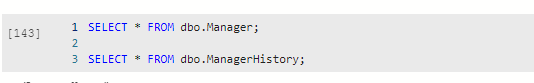
\includegraphics[width=7cm]{./Imagenes/s4}
		\end{center}
		\end{figure}   

                      \begin{figure}[H]
		\begin{center}
		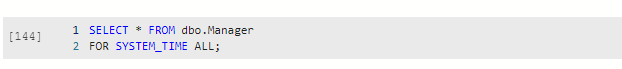
\includegraphics[width=7cm]{./Imagenes/s5}
		\end{center}
		\end{figure}   
         \item Verificar que el resultado sea el siguiente.
                     \begin{figure}[H]
		\begin{center}
		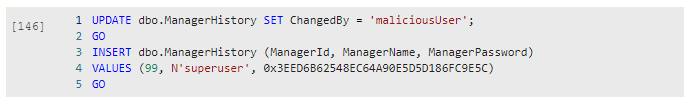
\includegraphics[width=7cm]{./Imagenes/s7}
		\end{center}
		\end{figure}   
\subsection{Creando un contenedor con Microsoft SQL Server para Linux}
	\item En la ventana de PowerShell, escribir el siguiente comando:"docker search mssql      
	\item El resultado deberá ser algo similar a lo siguiente.
                     \begin{figure}[H]
		\begin{center}
		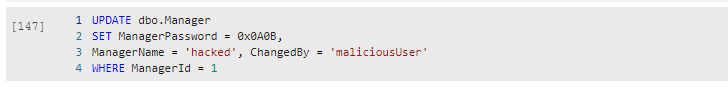
\includegraphics[width=15cm]{./Imagenes/s8}
		\end{center}
		\end{figure}   
	\item Ahora ejecutar el comando:"docker pull microsoft/mssql-server-linux"
	\item Lo cual descargará la imagen del contenedor de Microsoft SQL Server en un servidor Linux
                     \begin{figure}[H]
		\begin{center}
		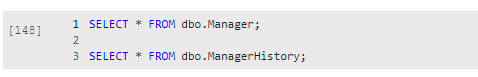
\includegraphics[width=15cm]{./Imagenes/s9}
		\end{center}
		\end{figure}   
          \item Proceder a verificar la imagen con el siguiente comando:" docker images"
	\item Lo cual deberá visualizar lo siguiente:
                     \begin{figure}[H]
		\begin{center}
		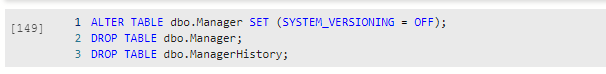
\includegraphics[width=15cm]{./Imagenes/s10}
		\end{center}
		\end{figure}   
	\item Seguidamente ejecutar el comando:
                      \begin{figure}[H]
		\begin{center}
		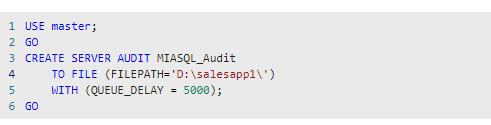
\includegraphics[width=15cm]{./Imagenes/s11}
		\end{center}
		\end{figure}   
	\item Como respuesta se visualizará un ID que corresponde al contenedor:
                     \begin{figure}[H]
		\begin{center}
		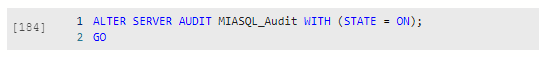
\includegraphics[width=15cm]{./Imagenes/s12}
		\end{center}
		\end{figure}   
           \item Verificar que el contenedor se este ejecutando correctamente mediante el comando:" docker ps"       
	\item Si se visualiza un cuadro de dialogo de permisos relacionados al firewall Windows, Aceptarlo para realizar la conexión.El resultado será similar al siguiente:
                     \begin{figure}[H]
		\begin{center}
		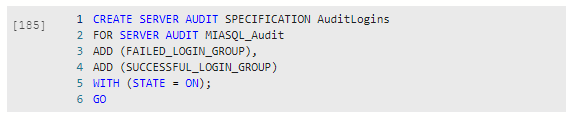
\includegraphics[width=15cm]{./Imagenes/s13}
		\end{center}
		\end{figure}   
	\item . Esperar unos segundos e iniciar la aplicación Microsoft SQL Server Management Studio, y conectar con los
siguientes datos:
                      \begin{figure}[H]
		\begin{center}
		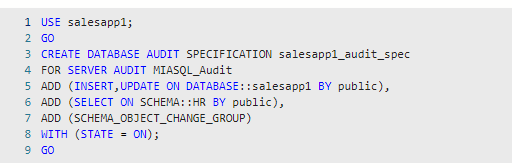
\includegraphics[width=15cm]{./Imagenes/s14}
		\end{center}
		\end{figure}   
	\item Iniciar una nueva consulta, escribir y ejecutar lo siguiente:
                     \begin{figure}[H]
		\begin{center}
		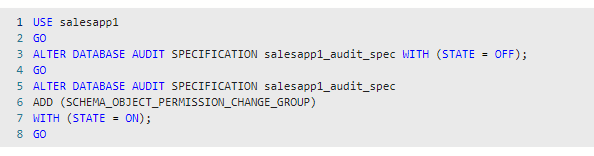
\includegraphics[width=15cm]{./Imagenes/s15}
		\end{center}
		\end{figure}   
          \item Deberá retornar algo similar a lo siguiente:
                     \begin{figure}[H]
		\begin{center}
		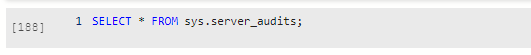
\includegraphics[width=15cm]{./Imagenes/s16}
		\end{center}
		\end{figure}   
	\item Cerrar la aplicación Microsoft SQL Server Management Studio.
	\item En PowerShell ejecutar el siguiente comando:" docker rm -f SQLLNX01"
                     \begin{figure}[H]
		\begin{center}
		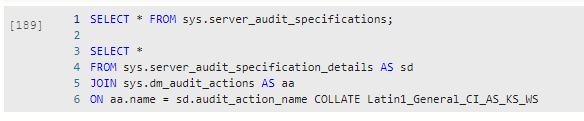
\includegraphics[width=15cm]{./Imagenes/s17}
		\end{center}
		\end{figure}   
	\item Verificar la eliminación del contenedor con ejecutando: docker ps
                    \begin{figure}[H]
		\begin{center}
		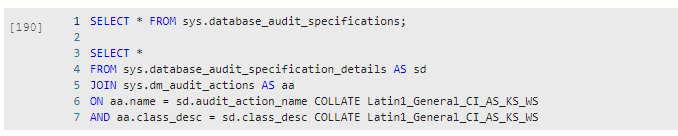
\includegraphics[width=15cm]{./Imagenes/s18}
		\end{center}
		\end{figure}   
\subsection{ Adicionando persistencia}
	\item En PowerShell ejecutar el siguiente comando.
                     \begin{figure}[H]
		\begin{center}
		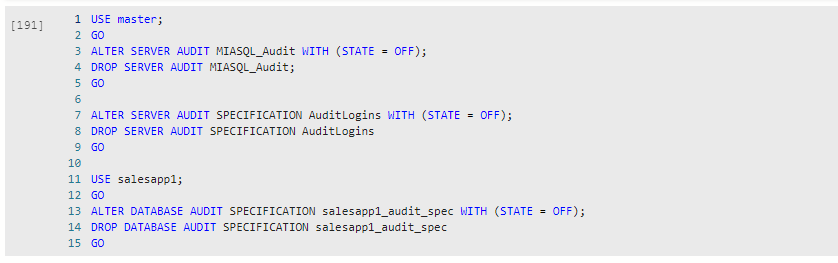
\includegraphics[width=15cm]{./Imagenes/s19}
		\end{center}
		\end{figure}   
          \item luego visualizara la siguiente ventana  ingresamos las credenciales.
                     \begin{figure}[H]
		\begin{center}
		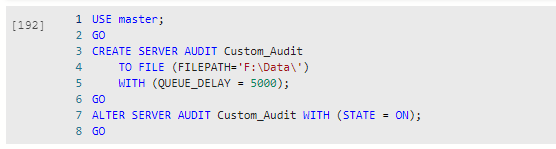
\includegraphics[width=15cm]{./Imagenes/s20}
		\end{center}
		\end{figure}   
	\item Como respuesta se visualizará un ID que corresponde al contenedor:
                     \begin{figure}[H]
		\begin{center}
		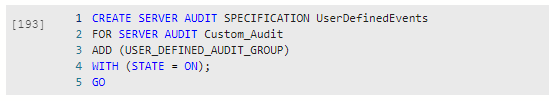
\includegraphics[width=15cm]{./Imagenes/s21}
		\end{center}
		\end{figure}   
	\item Verificar que el contenedor se este ejecutando correctamente mediante el comando:
                     \begin{figure}[H]
		\begin{center}
		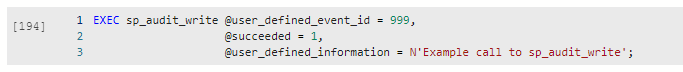
\includegraphics[width=15cm]{./Imagenes/s22}
		\end{center}
		\end{figure}   
           \item Esperar unos segundos e iniciar la aplicación Microsoft SQL Server Management Studio, y conectar con los siguientes datos:
                     \begin{figure}[H]
		\begin{center}
		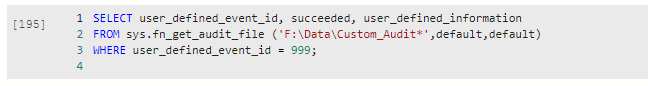
\includegraphics[width=15cm]{./Imagenes/s23}
		\end{center}
		\end{figure}   
	\item Generar una base de datos de prueba en la aplicación Microsoft SQL Server Management Studio, según la siguiente imagen mediante el siguiente script:
                     \begin{figure}[H]
		\begin{center}
		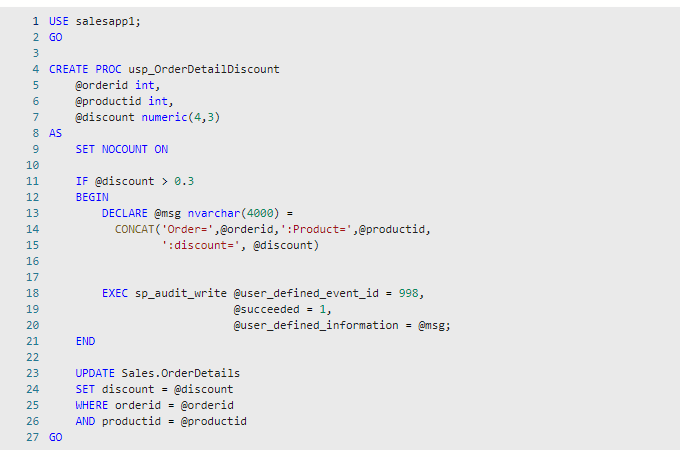
\includegraphics[width=15cm]{./Imagenes/s24}
		\end{center}
		\end{figure}   
           \item Verificar el contenido la carpeta DATALNX
                     \begin{figure}[H]
		\begin{center}
		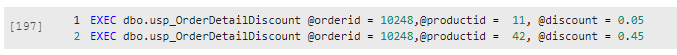
\includegraphics[width=15cm]{./Imagenes/s25}
		\end{center}
		\end{figure}   
           \item En PowerShell ejecutar el siguiente comando:"docker rm -f SQLLNX02"
                      \begin{figure}[H]
		\begin{center}
		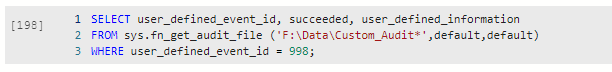
\includegraphics[width=15cm]{./Imagenes/s26}
		\end{center}
		\end{figure}   
	\item Verificar la eliminación del contenedor con ejecutando:"docker ps"
                    \begin{figure}[H]
		\begin{center}
		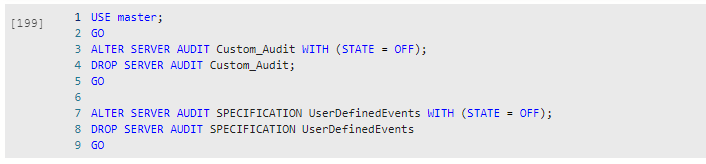
\includegraphics[width=15cm]{./Imagenes/s27}
		\end{center}
		\end{figure}   
\item antes se debe compartir o elnazar la carpeta  con Docker
                    \begin{figure}[H]
		\begin{center}
		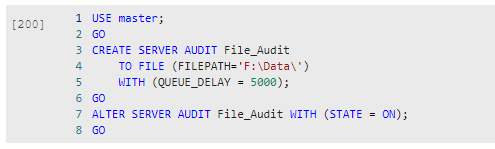
\includegraphics[width=15cm]{./Imagenes/s28}
		\end{center}
		\end{figure}   
\subsection{ Creando un contenedor con Microsoft SQL Server para Windows}
	\item En el icono de Docker en el área de notificación, hacer click con el botón derecho y utilizar la opción Switch to Windows Containers. Esperar a que Docker se reinicie.
                      \begin{figure}[H]
		\begin{center}
		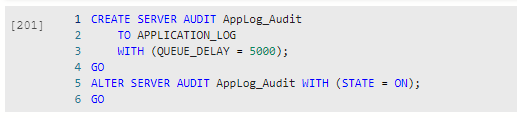
\includegraphics[width=10cm]{./Imagenes/s29}
		\end{center}
		\end{figure}   
                      \begin{figure}[H]
		\begin{center}
		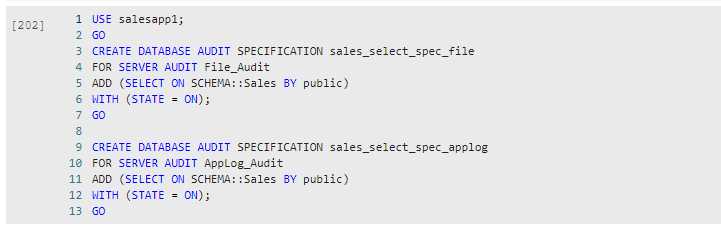
\includegraphics[width=10cm]{./Imagenes/s30}
		\end{center}
		\end{figure}   
	\item En la ventana de PowerShell, escribir el siguiente comando:"docker search mssql"           
                       \begin{figure}[H]
		\begin{center}
		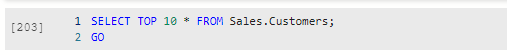
\includegraphics[width=15cm]{./Imagenes/s31}
		\end{center}
		\end{figure}   
          \item Ejecutar el siguiente comando; lo cual descargará la imagen del contenedor de Microsoft SQL Server en un servidor Linux.
		\begin{figure}[H]
		\begin{center}
		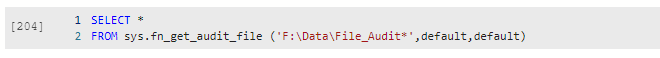
\includegraphics[width=15cm]{./Imagenes/s32}
		\end{center}
		\end{figure}  
         \item Proceder a verificar la imagen con el siguiente comando:
		\begin{figure}[H]
		\begin{center}
		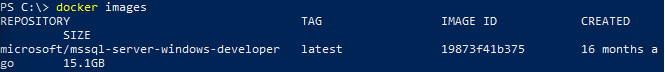
\includegraphics[width=15cm]{./Imagenes/c2}
		\end{center}
		\end{figure}  
          \item Seguidamente ejecutar el comando; como respuesta se visualizará un ID que corresponde al contenedor
		\begin{figure}[H]
		\begin{center}
		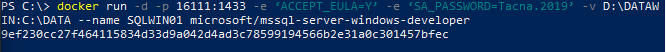
\includegraphics[width=15cm]{./Imagenes/c3}
		\end{center}
		\end{figure}  
          \item Repetir el paso 10 y verificar que el contenedor este ejecutándose
		\begin{figure}[H]
		\begin{center}
		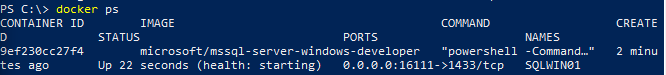
\includegraphics[width=15cm]{./Imagenes/c4}
		\end{center}
		\end{figure}  
          \item Repetir el paso 11 y conectar al servidor
		\begin{figure}[H]
		\begin{center}
		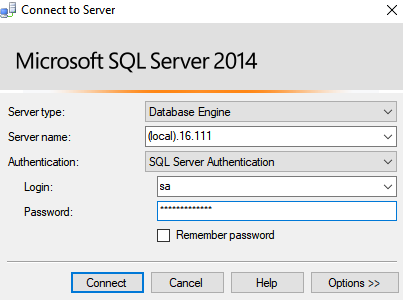
\includegraphics[width=15cm]{./Imagenes/c5}
		\end{center}
		\end{figure}  
         \item Iniciar una nueva consulta, escribir y ejecutar lo siguiente:
		\begin{figure}[H]
		\begin{center}
		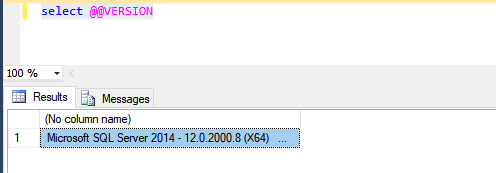
\includegraphics[width=10cm]{./Imagenes/c6}
		\end{center}
		\end{figure}  
          \item Generar una base de datos de prueba en la aplicación Microsoft SQL Server Management Studio
		\begin{figure}[H]
		\begin{center}
		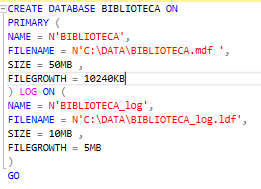
\includegraphics[width=10cm]{./Imagenes/c7}
		\end{center}
		\end{figure}  
          \item Verificar el contenido de la carpeta DATAWIN
		\begin{figure}[H]
		\begin{center}
		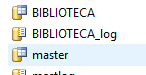
\includegraphics[width=12cm]{./Imagenes/c8}
		\end{center}
		\end{figure}  
         \item En PowerShell ejecutar el siguiente comando y verificar la eliminación del contenedor con ejecutando
		\begin{figure}[H]
		\begin{center}
		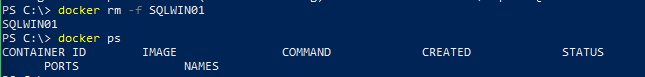
\includegraphics[width=15cm]{./Imagenes/c9}
		\end{center}
		\end{figure}  
          \item Cerrar la aplicación Microsoft SQL Server Management Studio.
       
\end{itemize}
		
\section{Analisis Interpretacioes y Resultados} 


\subsection{ Actividades Encargadas}
	\begin{itemize}
		\item ¿Con qué comando(s) exportaría la imagen de Docker de Microsoft SQL Server a otra PC o servidor?
                      \begin{figure}[H]
		\begin{center}
		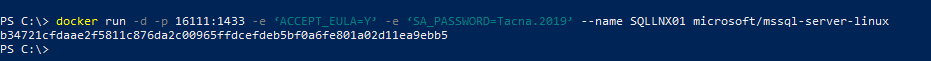
\includegraphics[width=15cm]{./Imagenes/6}
		\end{center}
		\end{figure} 
		\item ¿Con qué comando(s) podría generar dos volúmenes para un contenedor para distribuir en un volumen el Archivo de Datos (.mdf) y en otro el Archivo Log (.ldf)? 
                     \begin{figure}[H]
		\begin{center}
		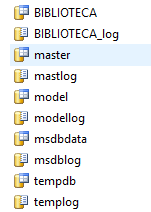
\includegraphics[width=7cm]{./Imagenes/18}
		\end{center}
		\end{figure} 
		\item Genere un nuevo contenedor y cree la base de datos con las siguientes características.
                      \begin{figure}[H]
		\begin{center}
		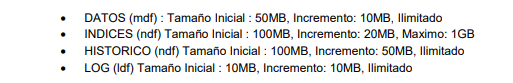
\includegraphics[width=7cm]{./Imagenes/30}
		\end{center}
		\end{figure} 
		\item  ¿Cuál sería el script SQL que generaría esta base de datos?
\begin{figure}[H]
		\begin{center}
		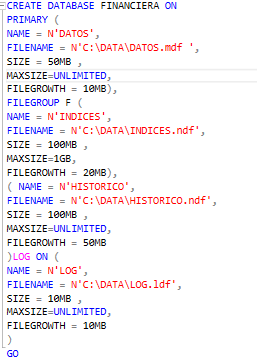
\includegraphics[width=10cm]{./Imagenes/t4}
		\end{center}
		\end{figure}
	\end{itemize}




\section{Concluciones}
\begin{itemize}
	\item En conclusión hemos observado y experimentado con docker, y nos resulta que es muy util al momento de instalar multiples bases de datos y que no existe la necesidad de armar o instalar múltipler ordenadores físicos o virtuales.
	
	\item Para concluir cabe destacar que los contenedores Docker comparten sus sistemas operativos para ser ejecutados como procesos aislados independientemente del sistema operativo de la máquina host. Docker se enorgullece, según sus propias palabras, de que sus contenedores se "pueden ejecutar en cualquier máquina, en cualquier infraestructura y en cualquier nube". La portabilidad, flexibilidad y simplicidad que esto permite son las razones fundamentales que explican por qué Docker ha sido capaz de crear tanta captación en tan poco tiempo.
\end{itemize}

\newpage

\section{WebGrafias} 

\begin{itemize}
	\item https://www.redhat.com/es/topics/containers/what-is-docker
	\item https://www.campusmvp.es/recursos/post/los-beneficios-de-utilizar-docker-y-contenedores-a-la-hora-de-programar.aspx
\end{itemize}




\end{document}
